In the seminal paper by Einstein \cite{einsteinUberErzeugungUnd1905}, that laid foundations to Quantum Mechanics, Einstein postulated that light is made of discrete quanta of energy $E = h\nu$ to explain the observations by Hertz and J.J. Thompson; explaining the photoelectric effect. The effect can be described by the Equation \ref{eq:photoelectric} where $E_e$ the emitted kinetic energy, $h$ is the plank's constant, $\nu$ the frequency of the incoming photon and  $\phi$ the material-specific work function (also known as binding energy). 

\begin{equation}\label{eq:photoelectric}
    E_e = h\nu - \phi
\end{equation}

The equation describes how incident photons on a surface eject photoelectrons, provided the photon energy $h\nu$ exceeds $\phi$. This also highlights that the emitted kinetic energy $E_e$ does not depend on the photon flux (photon counts per second). However, the flux increases the total amount of electrons released from the material.

It is then apparent that the binding energy of electrons can be found by irradiating light onto the material and measuring the $E_e$ of photoelectrons. \gls{PES}, is exactly such a technique that leverages this principle to probe the electronic structure of materials. While the above equation describes at what energies electron come out, it does not explain why 



A complete treatment of photoemission process needs the quantum theory of light-matter interaction, and this shall be introduced where necessary. 

\section{Light-Matter Interaction}\label{section:light-matter-interaction}
Where a complete description is not always necessary.

\section{Light Sources}\label{section:light-sources}
To perform \gls{PES}, it is imperative to first look at what the source of the electromagnetic radiation is necessary. The source needs to be monochromatic\footnote{Truly monochromatic radiation is physically impossible, and generally a range is considered.} and tunable, so that the only specific electrons are excited, allowing for precise measurement. Many materials of interest have binding energies lying in the UV to X-ray range. To measure not only the electronic states but also their dynamics, it becomes necessary to have a temporally coherent source.


\subsection{Laser}
The most ubiquitous of light sources--the laser--revolutionized experimental science as it enabled a vast range of phenomena to be precisely tested and observed, due to its high spatial and temporal coherence properties. A laser produces its light through a process known as stimulated emission, a process in which electrons, excited to higher energy states by an external energy source, emit photons as they return to lower energy states. These emitted photons, in turn, stimulate other electrons to release additional photons, leading to a cascade of coherent light. A process known as \gls{HHG} is used to generate ultrafast light of higher energies so that core electrons can be probed.  

\subsection{Synchrotron}
Particle accelerators, initially used for high energy physics experiments, which produce radiation as a byproduct of particles accelerating, found their use in spectroscopy. Soon, dedicated facilities providing extremely bright and tunable source of electromagnetic radiation emerged. One class of such facilities are known as Synchrotrons, which are named due to their cyclic design. Typically, bunches of electrons are accelerated by bending magnets, known as \glspl{undulator}, placed around a storage ring. These electrons are accelerated till they reach appropriate energies and provide a continuous source of radiation. Tangent to the ring, at certain points in the facility are beamlines which direct the radiation to the experimental end-stations, used to perform experiments in fields of life science, material science, and medicine to name a few.

There are several synchrotron facilities around the world, and in Germany such as BESSY II in Berlin, PETRA III at DESY campus in Hamburg.

\subsection{Free-Electron Laser}
TODO: Add more details about FELs
\begin{figure}
    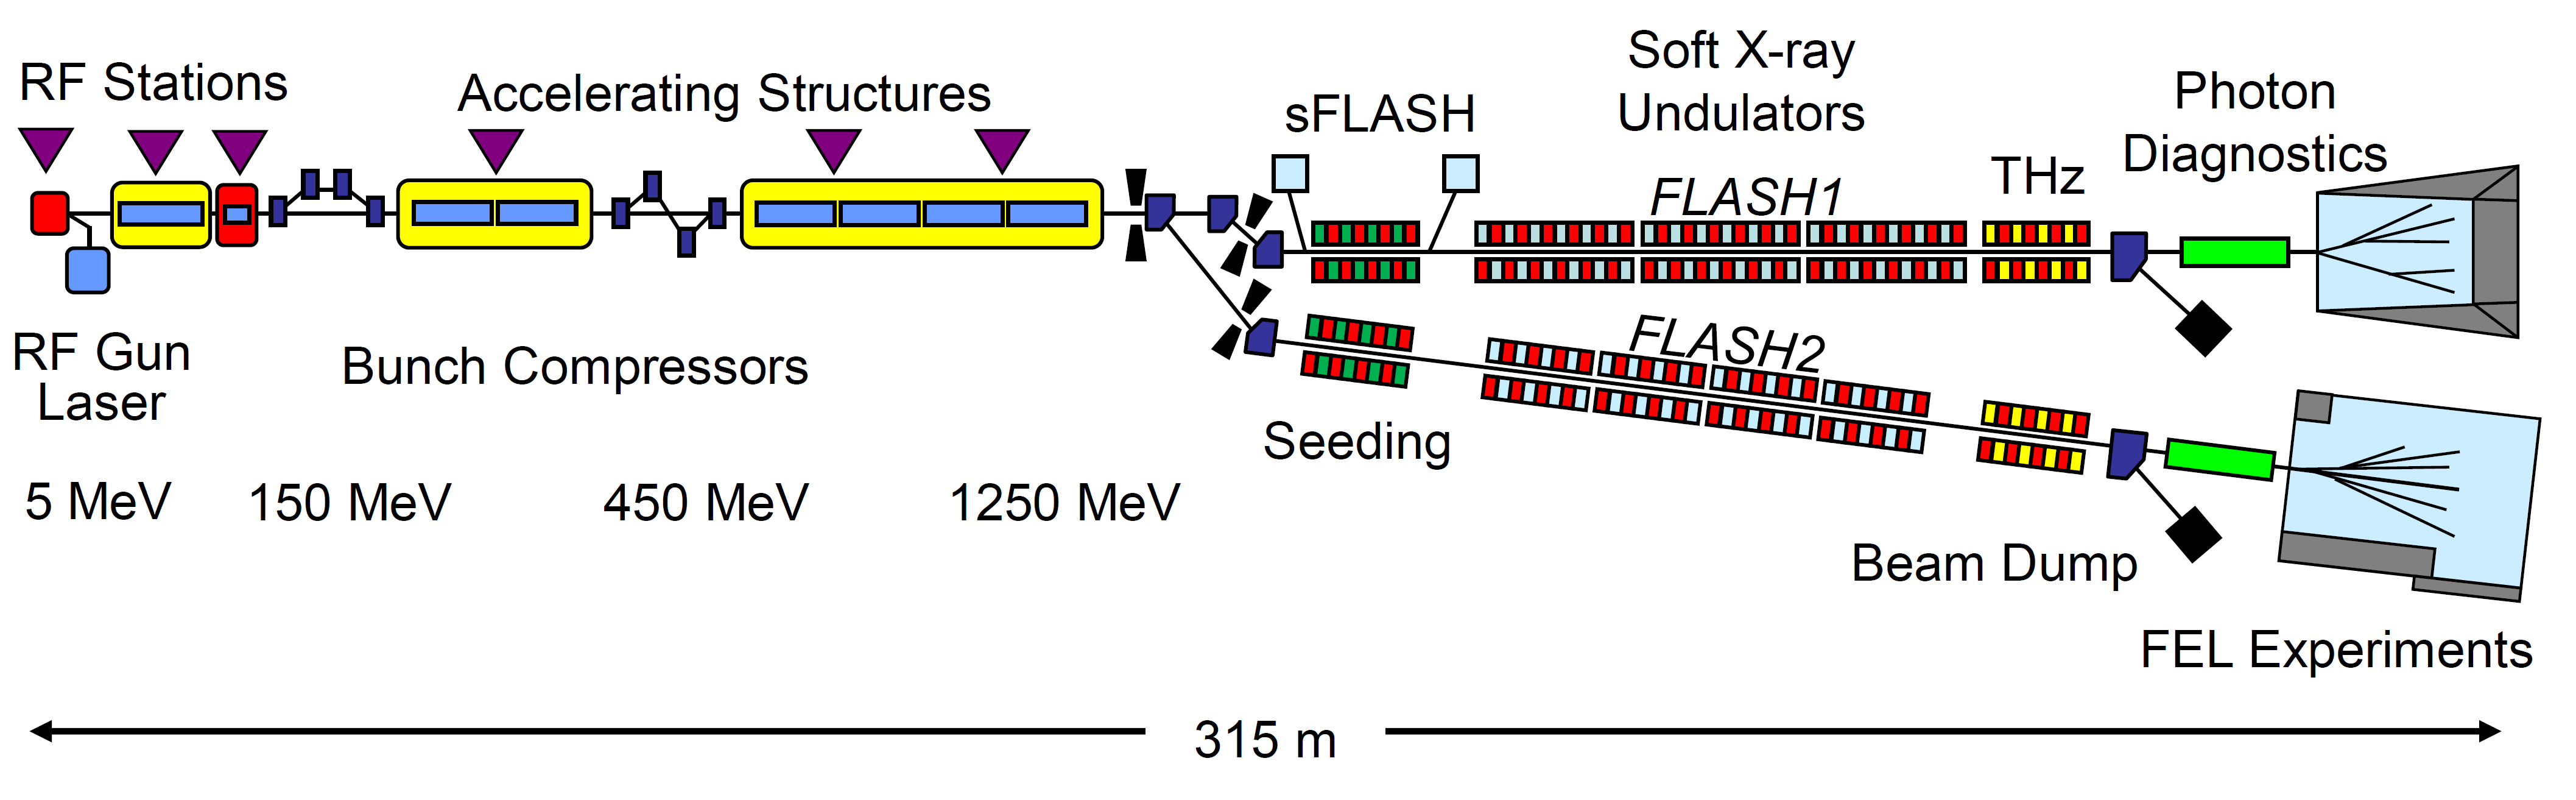
\includegraphics[width=1\linewidth]{images/flash_fel.png}
    \caption{Schematic view of \gls{FLASH} taken from \cite{faatzSimultaneousOperationTwo2016}.}
\end{figure}

While Synchrotrons are excellent sources of light for a multitude of experiments, they have limitations in terms of the temporal coherence of the light produced. \glspl{FEL} are a class of light sources that overcome this limitation. \glspl{FEL} are linear particle accelerators that produce radiation through spontaneous emission (see \cite[Chapters 5 and 10]{foxQuantumOpticsIntroduction2006} for a detailed explanation of spontaneous emission).

Unlike traditional lasers, FELs do not require a traditional optical cavity or gain medium. Instead, they use a linear particle accelerator to produce a bunched electron beam, which is then passed through an undulator. The undulator is a series of magnets that produce a periodic magnetic field, causing the electrons to oscillate and emit radiation. The emitted radiation interacts with the electrons, leading to microbunching, which produces coherent radiation.

The light produced is of high peak brightness and can be compressed to femtosecond pulse durations, making it an ideal source for studying ultrafast phenomena.

\gls{DESY} is a national research center in Germany that operates the \gls{FLASH} facility \cite{ackermannOperationFreeelectronLaser2007,tiedtkeSoftXrayFreeelectron2009}, which is a \gls{FEL} that produces soft X-ray radiation. The facility is used for a variety of experiments, including time-resolved studies of materials, and is equipped with a variety of end-stations to perform these experiments.


\begin{figure}
    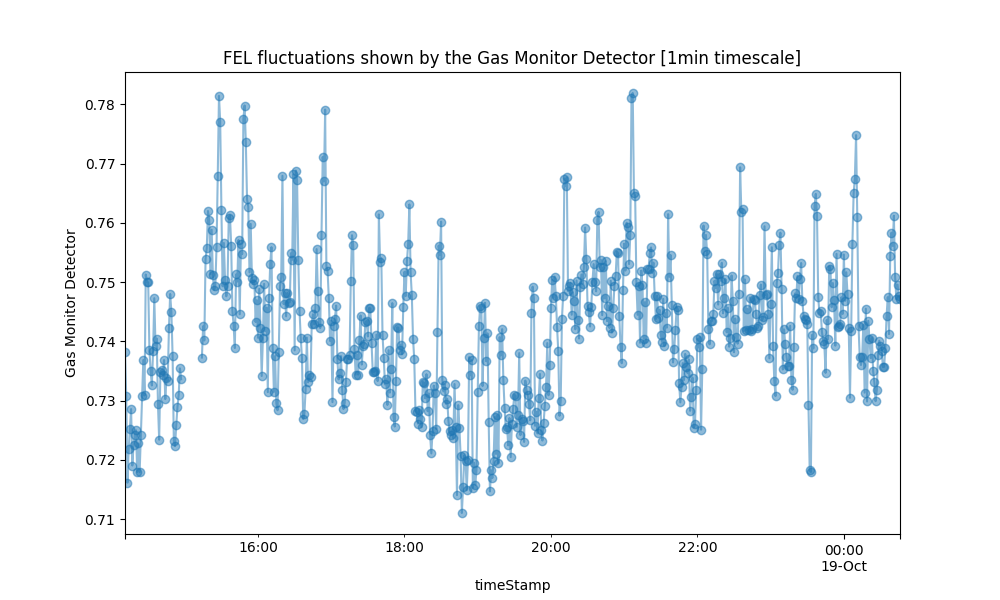
\includegraphics[width=1\linewidth]{images/2024-08-16-13-56-32.png}
\end{figure}


\section{HEXTOF instrument at FLASH}
A variety of photoemission spectrometers can be devised depending on which parameters are varied and what is measured. Naturally, the most basic setup would measure the energy of the emitted electron as described in equation \ref{eq:photoelectric}, but it is also common to measure the surface parallel momentum ($k_x$, $k_y$)

the whole process of excitation, transport, and emission is treated as a single coherent process using the formalism of quantum mechanics. This approach incorporates the electronic structure, electron-electron interactions, and the surface barrier in a unified way, and describes the photoemission intensity  I(E, $k_x$, $k_y$)  as:

% I(E, k_x, k_y) \propto |\langle \psi_f | \mathbf{A} \cdot \mathbf{p} | \psi_i \rangle|^2 \delta(E - E_f)

% where:

% 	•	 \psi_i  and  \psi_f  are the initial and final electron wavefunctions.
% 	•	 \mathbf{A} \cdot \mathbf{p}  is the interaction term representing the coupling between the electron and the incident photon (with vector potential  \mathbf{A}  and momentum operator  \mathbf{p} ).
% 	•	The delta function  \delta(E - E_f)  ensures energy conservation.


The \gls{HEXTOF} instrument is capable of performing time- and momentum-resolved photoemission studies 
\begin{figure}
    \centering
    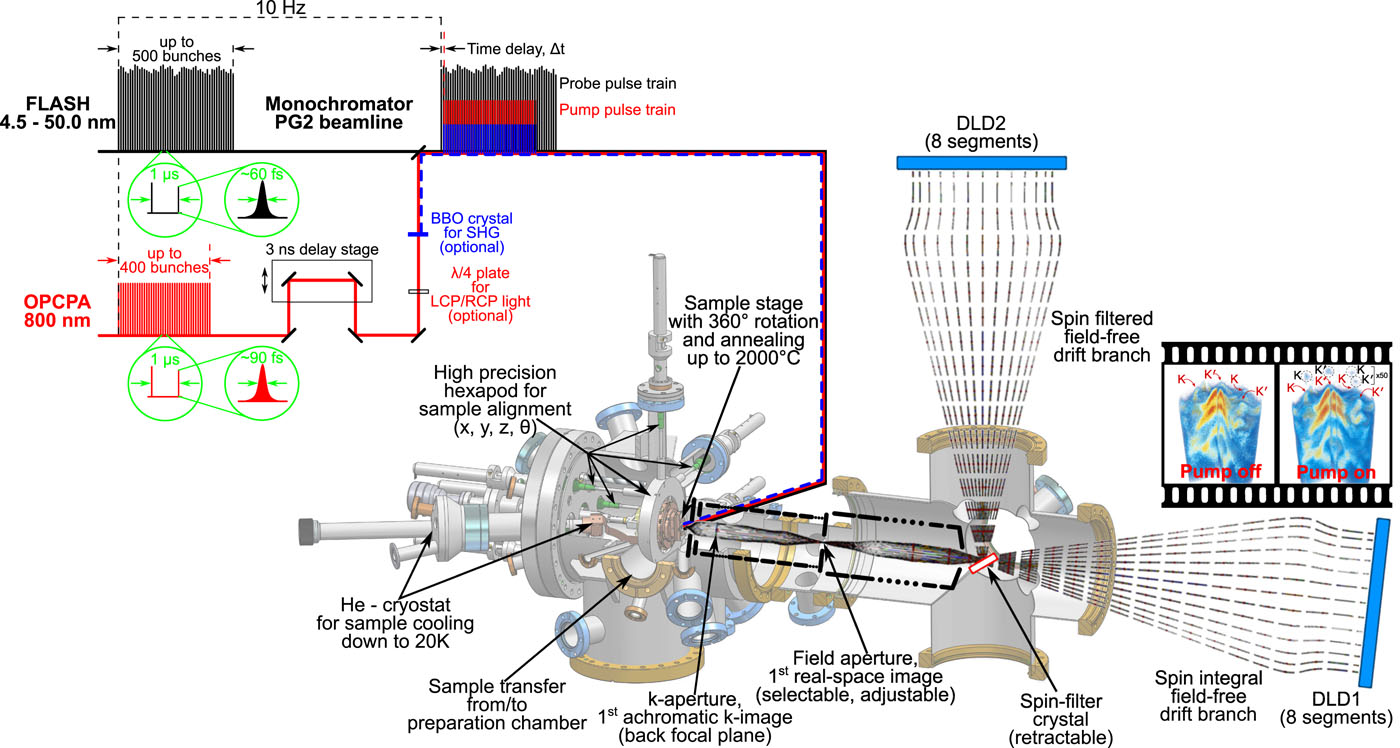
\includegraphics[width=1\linewidth]{images/2024-08-27-10-50-01.png}
    \caption{HEXTOF taken from \cite{kutnyakhovTimeMomentumresolvedPhotoemission2020}}
    % \label{fig:enter-label}
\end{figure}

\subsection{Delay Line Detectors}
The 3D detection scheme used in the \gls{HEXTOF} instrument consists of a \gls{DLD} and a \gls{TOF} tube. The \gls{DLD} is made of a \gls{MCP} for electron amplification and meanders to 

A Delayline Detector (DLD) operates by using a serpentine wire arrangement (meanders) positioned behind a micro-channel plate (MCP) for electron amplification. When particles (photons, ions, electrons) hit the MCP, they generate an electron cloud that induces electrical pulses in the meanders, allowing for precise time measurement of the hit position. This enables the reconstruction of the impact location and provides absolute time measurements relative to an external clock signal, processed by fast electronics and a time-to-digital converter (TDC).

\begin{figure}
    \centering
    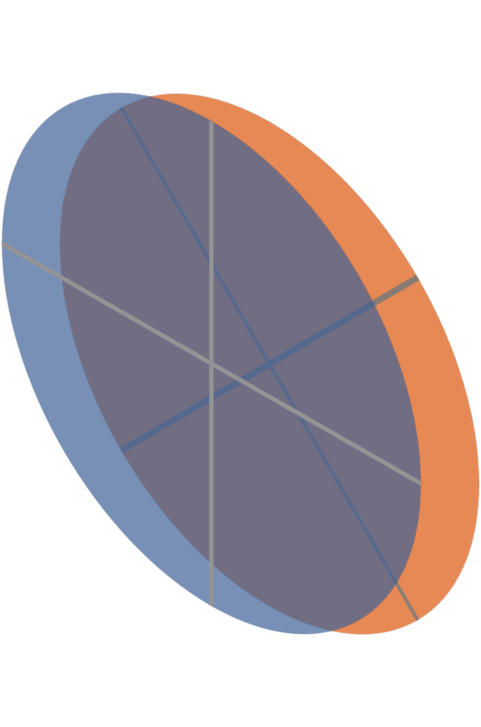
\includegraphics[width=0.3\linewidth]{images/sectors_figure.pdf}
    \caption{Schematic of the 2-layered DLD. The detector is divided into 2 layers, each with 4 sectors.}
    \label{fig:sectors}
\end{figure}

%images/chessy_deblurring_merged_events.png
\begin{figure}
    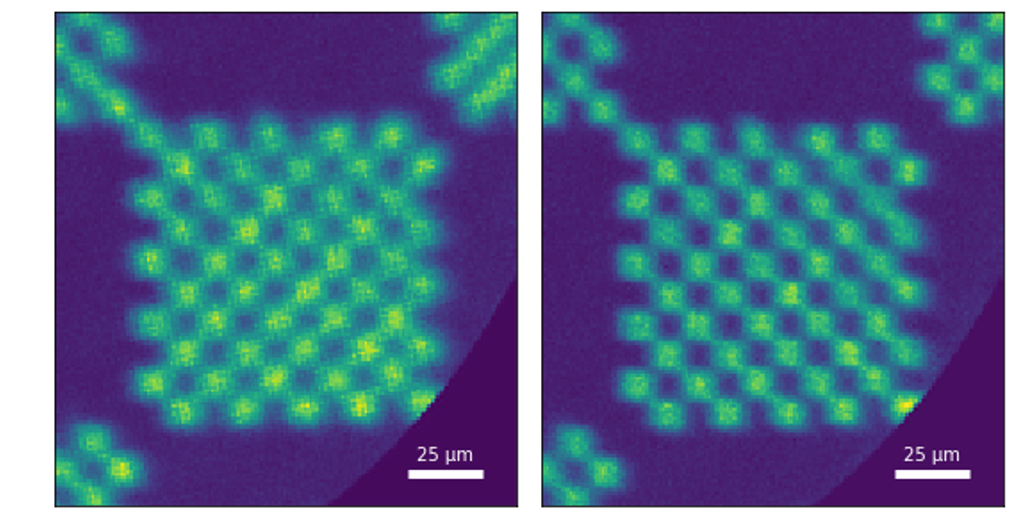
\includegraphics[width=1\linewidth]{images/chessy_deblurring_merged_events.png}
\end{figure}

\section{Binning as means of Imaging}
digital imaging from lecture
sampling etc
Binning is a way to find underlying distribution.


\section{Describing the data GdW, WSe2, GrIr, and new one}

\section{Creating the dataset Corrections Calibrations etc}\label{section:datasets}
\begin{figure}
    \centering
    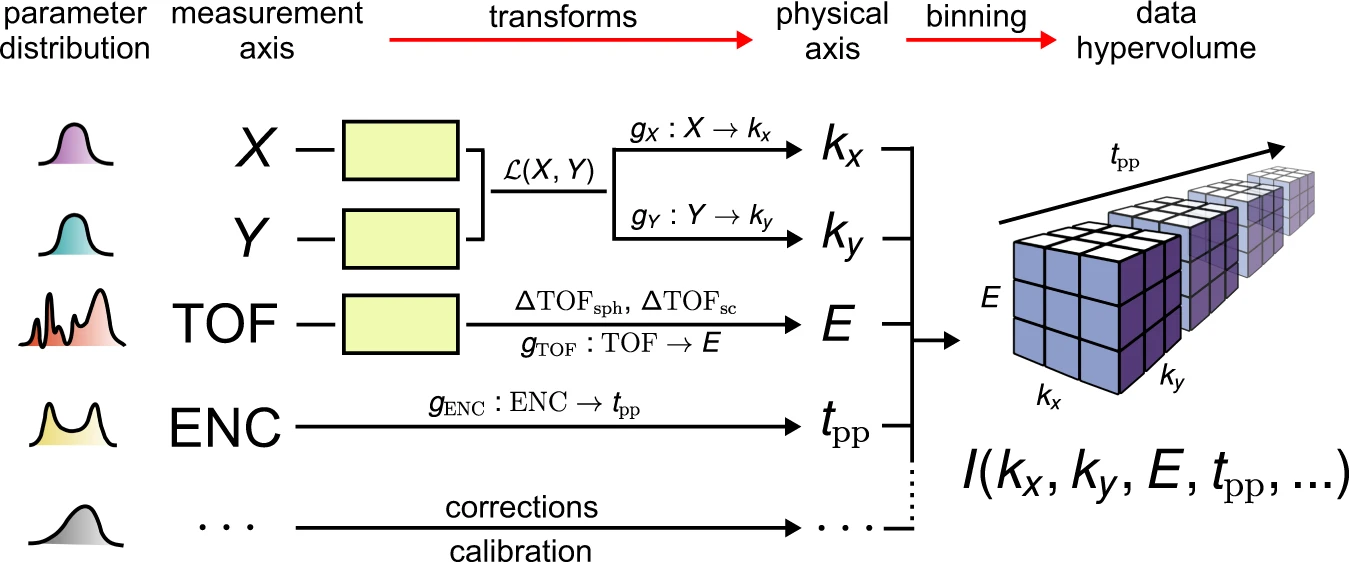
\includegraphics[width=1\linewidth]{images/2024-08-25-22-36-44.png}
    \caption{MPES taken from \cite{xianOpensourceEndtoendWorkflow2020}}
    % \label{fig:enter-label}
\end{figure}


Since the \gls{GrIr} dataset has the highest counts recorded compared ($\approx$186 M) to all our datasets, we will use the full dataset as ground truth and subsets of the single event data as noisy observations.